% Created 2022-08-13 Sat 10:08
% Intended LaTeX compiler: pdflatex
\documentclass[smaller, aspectratio=1610]{beamer}
\usepackage[utf8]{inputenc}
\usepackage[T1]{fontenc}
\usepackage{graphicx}
\usepackage{longtable}
\usepackage{wrapfig}
\usepackage{rotating}
\usepackage[normalem]{ulem}
\usepackage{amsmath}
\usepackage{amssymb}
\usepackage{capt-of}
\usepackage{hyperref}
\setbeamertemplate{navigation symbols}{}
\usepackage{verbatim, multicol, tabularx}
\usepackage{sourcecodepro}
\usepackage[T1]{fontenc}
\usepackage{amsmath,amsthm, amssymb, latexsym, listings, qtree}
\lstset{extendedchars=\true, inputencoding=utf8, frame=tb, aboveskip=1mm, belowskip=0mm, showstringspaces=false, columns=flexible, basicstyle={\footnotesize\ttfamily}, numbers=left, frame=single, breaklines=true, breakatwhitespace=true, tabsize=4,  keywordstyle=\color{blue}, identifierstyle=\color{violet}, stringstyle=\color{teal}, commentstyle=\color{darkgray}}
\setbeamertemplate{footline}[frame number]
\hypersetup{colorlinks=true,urlcolor=blue}
\usetheme{default}
\date{}
\title{Introduction to Python}
\hypersetup{
 pdfauthor={},
 pdftitle={Introduction to Python},
 pdfkeywords={},
 pdfsubject={},
 pdfcreator={Emacs 28.1 (Org mode 9.5.2)},
 pdflang={English}}
\begin{document}

\maketitle

\section{Introduction to Computing with Python}
\label{sec:org6b2129d}

\begin{frame}[label={sec:org4482155}]{Computing}
\alert{\alert{Computing}} is any purposeful activity that marries the representation of some dynamic domain with the representation of some dynamic machine that provides theoretical, empirical or practical understanding of that domain or that machine.

-- Isbell, et. al., \alert{(Re)Defining Computing Curricula by (Re)Defining Computing}, SIGCSE Bulletin, Volume 41, Number 4, December 2009
\end{frame}


\begin{frame}[label={sec:org5e93fc0}]{Models, Languages, Machines}
Computing is fundamentally a modelling activity.

\begin{itemize}
\item A \alert{model} is a representation of some information, physical reality, or a virtual entity in a manner that can then be interpreted, manipulated, and transformed.
\item A \alert{language} is a means of representation.

\begin{itemize}
\item A language enables reasoning and manipulation of the model.
\end{itemize}

\item A computational \alert{machine} allows us to execute our models.

\begin{itemize}
\item Computational models are \alert{runnable}.
\end{itemize}
\end{itemize}

In this course we will learn the Python programming language, one of many programming languages in which computational models can be represented.
\end{frame}

\begin{frame}[label={sec:org6ebb52a}]{Python gives you wings!}
\begin{center}
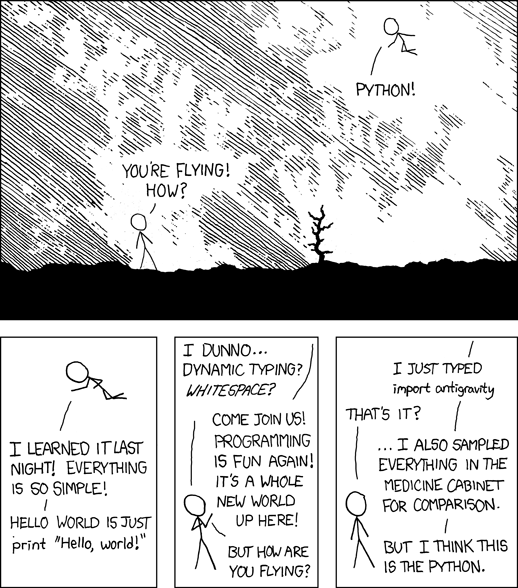
\includegraphics[height=.8\textheight]{./python.png}
\end{center}

\url{http://xkcd.com/353/}
\end{frame}

\begin{frame}[label={sec:org2750112}]{The Python Language}
\begin{itemize}
\item Python is a general-purpose programming language, meaning you can write any kind of program in Python

\begin{itemize}
\item A \alert{domain-specific language} is designed for one application. E.g., SQL is just for manipulating relational databases.
\end{itemize}

\item Python is interpreted, meaning you can run programs directly after you write them; you don’t have to compile programs to some intermediate form for the operating system or a virtual machine to execute.

\item Python is a great \href{https://www.python.org/doc/essays/omg-darpa-mcc-position/}{"glue"} language; Python programs often bring together disparate components to do a coherent task.

\begin{itemize}
\item One particular kind of glue is Python's killer feature for data science: easy to create Python bindings for libraries written in other languages
\item Data science libraries, e.g., NumPy, TensorFlow, are written high-performance languages like C and C++
\item Python provides a more comfortable way to use high-performance libraries
\end{itemize}
\end{itemize}

The coolest thing about Python \ldots{}
\end{frame}

\begin{frame}[label={sec:orgafe90e3}]{The Python Name}
\begin{center}
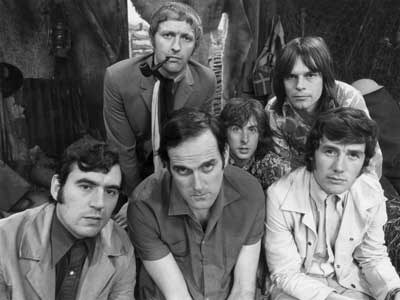
\includegraphics[height=.7\textheight]{./Flyingcircus_2.jpg}
\end{center}

\href{https://en.wikipedia.org/w/index.php?curid=6130072}{https://en.wikipedia.org/w/index.php?curid=6130072}

Python was named for Monty Python, of which Python’s creator, Guido van Rossum, is a big fan.
\end{frame}

\begin{frame}[label={sec:orga902983},fragile]{The \texttt{python3} Program}
 Practically speaking, Python is a program on your computer that interprets Python programs and statements.

\begin{itemize}
\item You can ask \texttt{python3} a question without running any Python code. For example, this is how you ask which version of Python is installed (Note: the \texttt{\$} character is the command prompt in the Unix Bash shell. The Windows command prompt is \texttt{C:\textbackslash{}>}.):

\lstset{language=sh,label= ,caption= ,captionpos=b,numbers=none}
\begin{lstlisting}
    $ python3 --version
    Python 3.8.10
\end{lstlisting}

If you get some other response, like command not found, then you haven’t properly installed Python.
\end{itemize}
\end{frame}

\begin{frame}[label={sec:orgf1b2c0b},fragile]{Executing Python Code}
 \begin{itemize}
\item You can run a Python program, which has a .py extension by convention:

\lstset{language=sh,label= ,caption= ,captionpos=b,numbers=none}
\begin{lstlisting}
    $ python3 myprogram.py
\end{lstlisting}

\item Or you can invoke the interactive Python shell (sometimes called REPL for "Read-Eval-Print Loop"):

\lstset{language=sh,label= ,caption= ,captionpos=b,numbers=none}
\begin{lstlisting}
    $ python3
    Python 3.8.10 (default, Jun  2 2021, 10:49:15)
    [GCC 9.4.0] on linux
    Type "help", "copyright", "credits" or "license" for more information.
    >>>
\end{lstlisting}

To exit the Python shell type Ctrl-D on Linux/Unix, or Ctrl-Z on Windows.
\end{itemize}
\end{frame}

\begin{frame}[label={sec:org59a86c8},fragile]{Hello, Python}
 Since Kernighan and Ritchie's "The C Programming Language" it's customary for your first program in a new language to be "Hello, world!"

\begin{itemize}
\item Open your text editor, paste the following code into a buffer (or tab or window or whatever your editor calls it), and save it as \texttt{hello.py}:

\lstset{language=Python,label= ,caption= ,captionpos=b,numbers=none}
\begin{lstlisting}
    print("Hello, world!")
\end{lstlisting}

\item Then open your command shell (terminal on Unix or CMD.exe on Windows), go to the directory where you saved \texttt{hello.py} and enter:

\lstset{language=sh,label= ,caption= ,captionpos=b,numbers=none}
\begin{lstlisting}
    $ python3 hello.py
\end{lstlisting}

Hello, world! will be printed to the console on the next line.
\end{itemize}
\end{frame}

\begin{frame}[label={sec:org3ed115a},fragile]{Interpreting Python Programs}
 What happens when we enter \texttt{python3 hello.py} at an operating system command shell prompt?

\begin{enumerate}
\item \texttt{python3} tells the OS to load the Python interpreter into memory and run it. \texttt{python} is the name of an executable file on your hard disk which your OS can find because its directory is on the \texttt{PATH}
\item We invoke \texttt{python} with a \alert{command line argument}, which \texttt{python3} reads after it starts running
\item Since the command line argument was the name of a file (\texttt{hello.py}), the \texttt{python3} loads the file and executes the Python code in it.
\end{enumerate}

A Python program, or script, is just a sequence of Python statements and expressions.
\end{frame}

\begin{frame}[label={sec:org87a8b92},fragile]{The Python REPL}
 Invoke the Python interactive shell by entering python at your command shell’s prompt without any arguments and type in the same line we put in hello.py:

\lstset{language=sh,label= ,caption= ,captionpos=b,numbers=none}
\begin{lstlisting}
$ python3
Python 3.8.10 (default, Jun  2 2021, 10:49:15)
[GCC 9.4.0] on linux
Type "help", "copyright", "credits" or "license" for more information.
>>>
\end{lstlisting}

\texttt{>>>} is the command prompt for the Python REPL.

\begin{itemize}
\item REPL stands for \alert{R} ead \alert{E} val \alert{P} rint \alert{L} oop:
\begin{enumerate}
\item \alert{Read} an expression or statement at the command prompt,
\item \alert{Evaluate} the expression or execute the statement,
\item \alert{Print} the result to the console, and
\item \alert{Loop} back to \alert{Read} step
\end{enumerate}
\end{itemize}

We’ll spend a lot of time in the REPL, but since this course is intended as a fast-paced introduction to Python for data analytics, we'll use \href{https://ipython.org/}{iPython}.
\end{frame}

\begin{frame}[label={sec:orgbef14ac},fragile]{iPython}
 Two modes:

\begin{itemize}
\item Interactive shell

\begin{itemize}
\item Replacement for \texttt{python} REPL
\end{itemize}

\item Jupyter notebook

\begin{itemize}
\item Interactive web-based documents mixing text, executable code, graphics
\end{itemize}
\end{itemize}

Before we proceed, make sure your computer is ready (OS shell):

\lstset{language=sh,label= ,caption= ,captionpos=b,numbers=none}
\begin{lstlisting}
$ pip install ipython
\end{lstlisting}
\end{frame}

\begin{frame}[label={sec:orgfa41bfb},fragile]{iPython Shell History}
 \lstset{language=sh,label= ,caption= ,captionpos=b,numbers=none}
\begin{lstlisting}
In [1]: ['Sage', 'Thyme', 'Oragano', 'Posh']
Out[1]: ['Sage', 'Thyme', 'Oragano', 'Posh']

In [2]: type(In[1])
Out[2]: str

In [3]: type(Out[1])
Out[3]: list

In [4]: spices = Out[1]

In [5]: spices
Out[5]: ['Sage', 'Thyme', 'Oragano', 'Posh']

In [6]: spices is Out[1]
Out[6]: True
\end{lstlisting}

\texttt{In} is a list, \texttt{Out} is a dict.
\end{frame}

\begin{frame}[label={sec:org10381ae},fragile]{iPython Help}
 Single \texttt{?} gives abbeviated version of python's \texttt{help}

\lstset{language=sh,label= ,caption= ,captionpos=b,numbers=none}
\begin{lstlisting}
In [7]: def add(a, b):
   ...:     """Return the result of + operation on a and b"""
   ...:     return a + b
   ...:
In [8]: add?
Signature: add(a, b)
Docstring: Return the result of + operation on a and b
File:      `/cs2316/<ipython-input-7-af5293282e78>
Type:      function
\end{lstlisting}

Double \texttt{??} gives source code, if available.

\lstset{language=sh,label= ,caption= ,captionpos=b,numbers=none}
\begin{lstlisting}
In [9]: add??
Signature: add(a, b)
Source:
def add(a, b):
    """Return the result of + operation on a and b"""
    return a + b
File:      `/cs2316/<ipython-input-7-af5293282e78>
Type:      function
\end{lstlisting}
\end{frame}

\begin{frame}[label={sec:org0d9c03b},fragile]{iPython Magic Commands}
 Special commands provided by iPython, prepended by \texttt{\%}.

\begin{itemize}
\item Run a Python script from within iPython:
\end{itemize}
\lstset{language=sh,label= ,caption= ,captionpos=b,numbers=none}
\begin{lstlisting}
In [35]: %run people.py
[<Stan, 2008-08-13, 150cm, 45kg>,
 <Kyle, 2008-02-25, 160cm, 50kg>,
 <Cartman, 2008-05-26, 140cm, 100kg>,
 <Kenny, 2009-07-30, 130cm, 40kg>]
\end{lstlisting}

\begin{itemize}
\item Get help with a magic command with \texttt{?}
\end{itemize}
\lstset{language=sh,label= ,caption= ,captionpos=b,numbers=none}
\begin{lstlisting}
In [2]: %cd?
Docstring:
Change the current working directory.

(content elided)

Usage:

  cd 'dir': changes to directory 'dir'.
(additional output elided)
\end{lstlisting}

Get a list of all magic commands with \texttt{\%lsmagic}
\end{frame}


\begin{frame}[label={sec:orgbd628ed},fragile]{iPython Shell Commands}
 Run shell commands by prepending with a \texttt{!}

\lstset{language=sh,label= ,caption= ,captionpos=b,numbers=none}
\begin{lstlisting}
In [27]: !ls *.py
fun.py		grades.py	maths.py	people.py	pp.py

In [28]: pyscripts = !ls *.py

In [29]: pyscripts
Out[29]: ['fun.py', 'grades.py', 'maths.py', 'people.py', 'pp.py']
\end{lstlisting}

iPython provides magic commands for most common shell commands.
\end{frame}


\begin{frame}[label={sec:org51036d7},fragile]{iPython Direcotry Bookmarking}
 Great timesaving feature: bookmark directories

\lstset{language=sh,label= ,caption= ,captionpos=b,numbers=none}
\begin{lstlisting}
In [3]: %pwd
Out[3]: '/home/chris/vcs/github.com/cs2316/cs2316.github.io/code'

In [4]: %cd
/home/chris

In [5]: %bookmark cs2316code `chris/vcs/github.com/cs2316/cs2316.github.io/code

In [6]: cd cs2316code
(bookmark:cs2316code) -> `chris/vcs/github.com/cs2316/cs2316.github.io/code
/home/chris/vcs/github.com/cs2316/cs2316.github.io/code
\end{lstlisting}
\end{frame}

\begin{frame}[label={sec:org0eaee52},fragile]{iPython Automagic commands}
 With \texttt{automagic} turned on, some shell commands can be run as if they were built into iPython:

\lstset{language=sh,label= ,caption= ,captionpos=b,numbers=none}
\begin{lstlisting}
In [22]: pwd
Out[22]: '/Users/chris/cs2316'

In [23]: ls *.py
fun.py     grades.py  maths.py   people.py  pp.py
\end{lstlisting}

\begin{itemize}
\item Toggle automagic on and off with \texttt{\%automagic}.

\item These commands work with automagic:

\begin{itemize}
\item \texttt{\%cd}, \texttt{\%cat}, \texttt{\%cp}, \texttt{\%env}, \texttt{\%ls}, \texttt{\%man}, \texttt{\%mkdir}, \texttt{\%more}, \texttt{\%mv}, \texttt{\%pwd}, \texttt{\%rm},  and \texttt{\%rmdir}
\end{itemize}
\end{itemize}
\end{frame}


\begin{frame}[label={sec:org73e1e70},fragile]{Timing Code in iPython}
 \lstset{language=sh,label= ,caption= ,captionpos=b,numbers=none}
\begin{lstlisting}
In [23]: import numpy as np

In [24]: pylist = list(range(1, 100000))

In [25]: nparray = np.arange(1, 1000000)

In [35]: %timeit _ = [x * 2 for x in pylist]
100 loops, best of 3: 7.89 ms per loop

In [37]: %timeit _ = nparray.copy() * 2
100 loops, best of 3: 3.76 ms per loop
\end{lstlisting}

Notice that I copied the Numpy array before applying the \texttt{* 2} operation to make the comparison to the Python list comprehension fair. You'll learn why when we discuss Numpy in the next lecture.
\end{frame}


\begin{frame}[label={sec:orgdb4a4d8}]{Conclusion}
\begin{itemize}
\item Python is an interpreted general purpose language

\item Python code can be run as programs or interactively in a Python REPL

\item Python is a great glue language

\item Python is fun!
\end{itemize}
\end{frame}
\end{document}